
\chapter{Service-Coverage Optimization \label{chap:06-Experimental-evaluation-the-service-coverage-problem}}

% First paragraph has no indentation.

\noindent The high-performance of PRATO, the radio-coverage simulation
framework presented in Chapter~\ref{chap:04-Framework-design-and-implementation},
allows dealing with big problem instances in a reduced amount of time.
Additionally, it enables tackling optimization problems that, because
of their size, are out-of-reach of traditional approaches, mainly
due to the computational-time complexity of their objective-function
evaluation.

In this chapter, the challenge is to exploit PRATO for solving one
of the classic optimization problems of radio networks: the service-coverage
problem. Considering the minimization of the total amount of pilot
power subject to a full coverage constraint, a novel optimization
approach is introduced. The presented method, based on parallel autonomous
agents, gives very good solutions to the problem in an acceptable
amount of time. The parallel implementation takes full advantage of
GPU hardware in order to achieve considerable speedup. The analysis
of the experimental results, considering six real-world, radio networks
of different sizes, studies solution-quality and performance aspects.

The content of this chapter extends the research work published by
the author in~\cite{Benedicic_Pilot.power.optimization:2010} and~\cite{Benedicic-A_GPU_based_parallel_agent_optimization_approach:2013}.
The rest of this chapter is organized as follows. Section~\ref{sec:06-Motivation}
gives a description of the coverage problem and its motivation from
the mobile operator's perspective. In Section~\ref{sec:06-Related-work},
a short overview of related research works is given, before formally
introducing the key elements of the service-coverage problem in Section~\ref{sec:06-Radio_network_model}.
The parallel-agent approach, as well as the strategies used for result
comparison, are presented in Section~\ref{sec:06-Optimization-approaches},
followed by the simulations and their analyses in Section~\ref{sec:06-Simulations}.


\section{Motivation \label{sec:06-Motivation}}

Solving the service-coverage problem for radio networks has received
a great deal of attention in the past years. Its complexity demands
the confluence of different skills in areas such as propagation of
radio signals, telecommunications and information systems, among others.

Even several decades after the launch of the first commercial GSM
network, service-coverage planning remains a key problem that all
mobile operators have to deal with. Its intricacy arises from the
wide range of different combinations of configuration parameters and
their evaluation-time complexity.

Regardless of the mobile technology used, e.g., GSM, UMTS or LTE,
a lower transmit power generates less interference, which, in turn,
translates into more capacity of the radio link (see Chapter~\ref{chap:02-Principles_of_mobile_radio_networks}).
Additionally, reducing the transmit-power usage is also related to
issues regarding human exposure to the electromagnetic fields generated
by BS antennas~\cite{Esposito_Genetic.optimization.for.optimum.3G.network.planning:2010}.
During the past few years, public opinion has been extremely sensitive
regarding this issue, and thus many countries have already imposed
safety standards to limit the electromagnetic field levels produced
by antennas in a given range.

From the UMTS perspective, minimizing pilot-power usage leaves more
power available for increased network capacity. This is especially
important if the traffic and other channels are configured relative
to the pilot channel~\cite{WCDMAforUMTS_RadioAccessForThirdGenerationMobileCommunications}.
Moreover, as the demand for internet access and data services increases~\cite{Cunningham_Network.growth.theory.and.evidence:2010},
so does the pressure on existing network infrastructure, making parameter
optimization the only viable solution in the short-term~\cite{Nawrocki-Understanding_UMTS_radio_network_modelling_and_optimisation:2006}.

\bigskip{}


The idea of using autonomous agents for optimization is not new. It
has proven to be a solid optimization approach for solving different
types of problems, not only within the area of radio networks~\cite{Cheung_Realtime.video.using.agent.over.3G.networks:2005,Esposito_Genetic.optimization.for.optimum.3G.network.planning:2010},
but also in other fields~\cite{Valcarce_Applying.FDTD.to.the.coverage.prediction.of.WiMAX:2009,Vasile_Hybrid.multiagent.approach.for.optimization:2009}.
The increased computational-time complexity, when dealing with big
problem instances, is tackled using a parallel, agent-based algorithm
on GPU. This minimizes the overhead when deploying a larger number
of agents working in parallel over the service area, only limited
by the amount of memory available on the GPU.


\section{Related work \label{sec:06-Related-work}}

There are several approaches in the literature that address the service-coverage
problem in radio networks~\cite{Amaldi-Radio_planning_and_coverage_optimization_of_3G_networks:2008,Nawrocki-Understanding_UMTS_radio_network_modelling_and_optimisation:2006,Siomina_Pilot.power.optimization:2004}.
Some of them even claim to achieve near-optimal solutions~\cite{Siomina:Minimum.pilot.power.for.service.coverage}.
As a matter of fact, most formulations are only useful for small network
instances and often fail when challenged with larger, real-world networks.

A genetic-algorithm approach for solving the service-coverage problem
for GSM networks was presented in~\cite{Lieska-Radion_coverage_optimization_with_genetic_algorithms:1998}.
The proposed solution is based on the physical distribution of BSs
in order to maximize coverage. The simulations were performed on a
test network with 40 candidate sites for BS antennas.

In~\cite{Siomina:Minimum.pilot.power.for.service.coverage}, Siomina
and Yuan considered the problem of minimizing the total amount of
pilot power for UMTS networks, subject to a full coverage constraint.
They tackled the problem with an iterative linear-programming approach,
reporting very good results for some test networks, containing from
15 to 65 base stations. The authors noted that bigger problem instances
could not be solved because of hardware constraints on the target
platform.

As for LTE networks, the service-coverage problem was addressed in~\cite{Thampi-A_sparse_sampling_algorithm_for_self_optimization_of_coverage_in_LTE:2012}.
The authors presented an algorithm, based on reinforcement learning,
to tackle three aspects of the coverage problem, i.e., coverage holes,
weak coverage and pilot pollution. The experimental simulations, performed
on 3 BSs, used different antenna-tilt configurations as the proposed
solutions.

The service-coverage problem, as presented in this chapter, corresponds
to achieving full coverage of the target area, without coverage holes.


\section{Radio-network model \label{sec:06-Radio_network_model}}

Extending the representation of a radio-network model from~\cite{Nawrocki-Understanding_UMTS_radio_network_modelling_and_optimisation:2006},
this section presents the definitions of all the elements included
in the mathematical model used for the simulations.

The goal here is to analyze the state of the network in a given situation,
i.e., a \textquoteleft{}snapshot\textquoteright{} at an arbitrary
instance. Radio-network planning tools, including the commercial ones,
typically rely on static analysis~\cite{Niemela-Performance_of_static_WCDMA_simulator:2005}.

A snapshot consists of a set of UEs having individual properties,
such as location, and equipment type that provides an estimate of
the average network behavior. The static approach inherently ignores
dynamic effects that influence the system, like fast power control,
but the analysis relies on having multiple independent snapshots to
produce an average behavior.

Another alternative is to consider using a dynamic tool for radio-network
planning~\cite{Hamalainen-Advanced_WCDMA_radio_network_simulator:1999,Hoppe-Fast_planning_of_efficient_WCDMA_radio_networks:2001}.
A dynamic simulation considers all Radio-Resource Management~(RRM\nomenclature[A]{RRM}{Radio-resource management})
functionality, as well as user mobility. However, when compared to
the static approach, a major disadvantage of the dynamic simulation
is the large computational time it requires. This clearly excludes
the possibility of achieving fast performance evaluations of a network,
which is one of the objectives of this thesis.

Considering that the performance of a static approach was demonstrated
to provide sufficiently accurate results compared to a fully dynamic
approach~\cite{RadioNetworkPlanningAndOptimisationForUMTS,Laiho-Verification_of_WCDMA_network_planning_prediction_with_dynamic_simulations:2001},
the former one is implemented in this work.

For additional information regarding mathematical models for radio
networks and signal propagation, see~\cite{RadioNetworkPlanningAndOptimisationForUMTS,Nawrocki-Understanding_UMTS_radio_network_modelling_and_optimisation:2006,Stuber-Principles_of_mobile_communication:2011}.


\subsection{Basic elements}

Consider a radio network with a set of antenna installations (cells),
$C$\nomenclature[S]{$C$}{Set of antenna installations (cells) in a mobile network}.
A RSG of a given resolution represents a geographical area, $A_{\mathrm{total}}$,
within which a set of UEs, $M$\nomenclature[S]{$M$}{Set of mobile devices or users of a mobile network},
is spatially distributed over the pixels of $A_{\mathrm{total}}$.
Further, $l_{cm}^{\downarrow}$\nomenclature[S]{$l_{cm}^{\downarrow}$}{Downlink attenuation factor between cell $c\in C$ and mobile $m\in M$}
is defined as the downlink attenuation factor between cell $c\in C$
and UE $m\in M$. Similarly, $l_{mc}^{\uparrow}$\nomenclature[S]{$l_{mc}^{\uparrow}$}{Uplink attenuation factor between mobile $m\in M$ and cell $c\in C$}
represents the uplink attenuation factor between UE $m$ and cell
$c$. The attenuation factor values are calculated by performing signal-propagation
predictions for every pair $(c,m)$, using the radio-propagation model
introduced in Section~\ref{sub:04-Radio_propagation_model}. These
predictions already include losses and gains from cabling, hardware,
and user equipment.

The amount of power allocated to the pilot signal of cell $c$ is
denoted as $p_{c}$\nomenclature[S]{$p_{c}$}{Pilot-power setting of cell $c\in C$},
and it can adopt any value from the sorted set of available pilot
power levels, $P_{c}=\{p_{c}^{1},p_{c}^{2},...,p_{c}^{k}\}$\nomenclature[S]{$P_{c}$}{Set of candidate pilot power settings for cell $c\in C$},
where $p_{c}^{k}$ is the maximum power.

Based on the introduced elements, the received pilot power from cell
$c$ to UE $m$ is $l_{cm}^{\downarrow}p_{c}$.


\subsection{Coverage}

A UE $m$ within the area $A_{\mathrm{covered}}$ is under service
coverage if at least one cell $c$ covers it. Cell coverage is provided
to a UE $m$ from a cell $c$ if its signal-to-interference ratio,
$\mathrm{SINR}(c,m)$\nomenclature[S]{$\mathrm{SINR}(c,m)$}{Signal-to-interference ratio from cell $c\in C$ to mobile $m\in M$},
at the RSG pixel where $m$ is located, is not lower than a given
threshold, $\gamma^{\mathrm{cov}}$\nomenclature[S]{$\gamma^{\mathrm{cov}}$}{Signal-to-interference ratio coverage threshold}:

\begin{equation}
\mathrm{SINR}(c,m)=\frac{l_{cm}^{\downarrow}p_{c}}{\mathrm{N}_{0}+\sum_{i\in C}l_{im}^{\downarrow}p_{i}}\ge\gamma^{\mathrm{cov}},\label{eq:06-Signal_to_interference_ratio}
\end{equation}


\noindent where $\mathrm{N}_{0}$\nomenclature[S]{$\mathrm{N}_0$}{Thermal noise}
is the thermal noise~\cite{RadioNetworkPlanningAndOptimisationForUMTS}.
For convenience, a binary function is defined to determine the coverage
of a UE $m$ by a cell $c$. So, for any pair $(c,m)$, the coverage
of UE $m$ by cell $c$ is defined as:

\begin{equation}
\mathrm{cov}(c,m)=\begin{cases}
1 & if\,\mathrm{SINR}(c,m)\ge\gamma^{\mathrm{cov}}\\
0 & otherwise
\end{cases}.
\end{equation}


\noindent \nomenclature[S]{$\mathrm{cov}(c,m)$}{Binary function to assert the coverage of a mobile $m\in M$ from a cell $c\in C$}

\noindent A set, denoted as $C_{m}$\nomenclature[S]{$C_{m}$}{Subset of cells, $C_m\subset C$, that cover a mobile $m\in M$},
$C_{m}\subset C$, contains all the cells covering a UE $m$. From
this set, the cell with the highest $\mathrm{SINR}(c,m)$ is referred
to as the best server, and denoted as $c_{m}^{*}$\nomenclature[S]{$c_{m}^*$}{Best-serving cell of mobile $m\in M$}.

\noindent Notice that the described radio-network model is easily
adaptable for different mobile technologies, e.g., GSM, UMTS and LTE.
For example, if solving the service-coverage problem for UMTS, it
would be reasonable to assume that all cells in the network operate
at maximum power, and adapt Equation~(\ref{eq:06-Signal_to_interference_ratio})
accordingly. This is, from the interference point of view, the worst-case
scenario~\cite{chen2008automated,Siomina:Minimum.pilot.power.for.service.coverage}.
This assumption guarantees that even under heavy user traffic full
coverage of the service area is maintained, due to the cell-breathing
principle~\cite{WCDMAforUMTS_RadioAccessForThirdGenerationMobileCommunications}.


\section{Problem definition}

In the problem of optimization of pilot powers for service coverage,
the objective is to find a set of pilot-power settings for all cells
in the network, such that the total pilot power used is minimized,
and a given service coverage criteria is fulfilled. In other words,
solving the service-coverage problem corresponds to finding the pilot
power levels $p_{c}$, for all cells $c\in C$, such that coverage
of at least $b$ UEs is guaranteed, while the total amount of pilot
power used is minimized. Here, full coverage of the service area is
being considered, thus $b=\vert M\vert$. Consequently, the optimization
objective is defined as follows:

\begin{equation}
P^{*}=\min\sum_{c\in C}p_{c},\, p_{c}\in P_{c}\label{eq:06-Objective_function}
\end{equation}


\noindent subject to

\begin{equation}
\frac{\sum_{m\in M}\mathrm{cov}(c_{m}^{*},m)}{b}=1.\label{eq:06-Coverage_constraint}
\end{equation}


\bigskip{}


It has been proved that the problem of pilot-power optimization for
full coverage of the service area is $NP$-hard, since it can be reduced
to the set-covering problem~\cite{Varbrand_Mathematical.programming.approach:2003}.
Consequently, as long as $P\neq NP$, it is unfeasible that a polynomial-time
algorithm exists, which is able to find an exact solution to this
problem.


\section{Optimization approaches \label{sec:06-Optimization-approaches}}

Since some of the analyzed problem instances are part of a real mobile
network deployed in Slovenia by Telekom Slovenije, d.d., there are
no references in the literature of other optimization techniques dealing
with exactly the same data set. For this reason, two different strategies
for setting the pilot power are being presented. They should provide
a basis for the comparison of the experimental results. The first
strategy is the attenuation-based pilot power, presented in~\cite{Siomina_Pilot.power.optimization:2004},
in which a pixel of the service area is always covered by the cell
with the maximum attenuation-factor value, i.e., the minimum path
loss. The second strategy is the presented parallel-agent approach,
based on ideas inspired by two-dimensional cellular automata~\cite{Sarkar_Cellular.automata.history:2000}
and metaheuristics~\cite{Talbi_Metaheuristics:2009}. A detailed
description is given in Section~\ref{sub:06-Parallel_agent_approach}.

Similar criteria for result comparison have also been used in~\cite{Siomina_Pilot.power.optimization:2004,Siomina:Minimum.pilot.power.for.service.coverage}.


\subsection{Attenuation-based approach}

The first heuristic for setting the pilot power of all cells in the
network is known as attenuation-based, since it relies on the downlink-attenuation
factor, $l_{cm}^{\downarrow}$. A UE located on some pixel of the
service area is always covered by the cell with the minimum path loss,
i.e., the highest $l{}_{cm}^{\downarrow}$ value. Whenever the maximum
available power, $p_{c}^{k}$, is the same for all the cells in the
network, this is equivalent to selecting the cell with the minimum
required pilot power to cover a UE $m$. Hence, under this assumption,
the cell $c$ covering UE $m$ is identified as:

\begin{equation}
p_{cm}^{\mathrm{att}}=\min p_{c}\,\forall c\in C\iff\mathrm{cov}(c,m)=1\label{eq:06-Attenuation_based-power}
\end{equation}


Picking the cells conforming to Equation~(\ref{eq:06-Attenuation_based-power})
and setting the pilot powers accordingly, full coverage of the service
area is achieved. The solution exhibits a total pilot power defined
as:

\begin{equation}
P^{\mathrm{att}}=\sum_{c\in C}\max p_{cm}^{\mathrm{att}}.
\end{equation}


The procedure to find a cell $c$ for every UE $m$ in the service
area consists in sorting, in descending order, all UEs by their attenuation-factor
values, $l_{cm}^{\downarrow}$. The solution is thus established by
the first $b$ UEs of the sorted sequence, taking the maximum pilot-power
setting for a cell into account, i.e., $p_{cm}^{\mathrm{att}}$.


\subsection{Parallel-agent approach \label{sub:06-Parallel_agent_approach}}

In the parallel-agent approach, a set of autonomous worker agents
explore the target geographical area, $A_{\mathrm{total}}$, in order
to optimize the pilot-power consumption. Each agent randomly moves
over the $A_{\mathrm{total}}$ as it dictates different changes to
the pilot power of the cells. PRATO, the radio-coverage framework
presented in Chapter \ref{chap:04-Framework-design-and-implementation},
performs the objective-function evaluations and radio-propagation
predictions based on the proposed changes of the agents.

The moving process during the optimization is strictly random. However,
several physical properties that are exclusive to the service-coverage
problem are being exploited during the exploration of the search space.
Additionally, whenever the current solution breaks any of the given
constraints, the optimization process is guided back to the space
of valid solutions, providing a mechanism for improving exploration
and escaping from local optima.

Because the behavior of the agents is independent between each other,
a parallel implementation is fairly straight-forward to achieve. Figure~\ref{fig:06-Architecture_of_the_system_on_GPU}
shows the architecture of the agent-optimization system. In this GPU-only
architecture, agents work in a parallel and autonomous manner, while
the evaluator reacts to their changes.

\begin{figure}
\centering

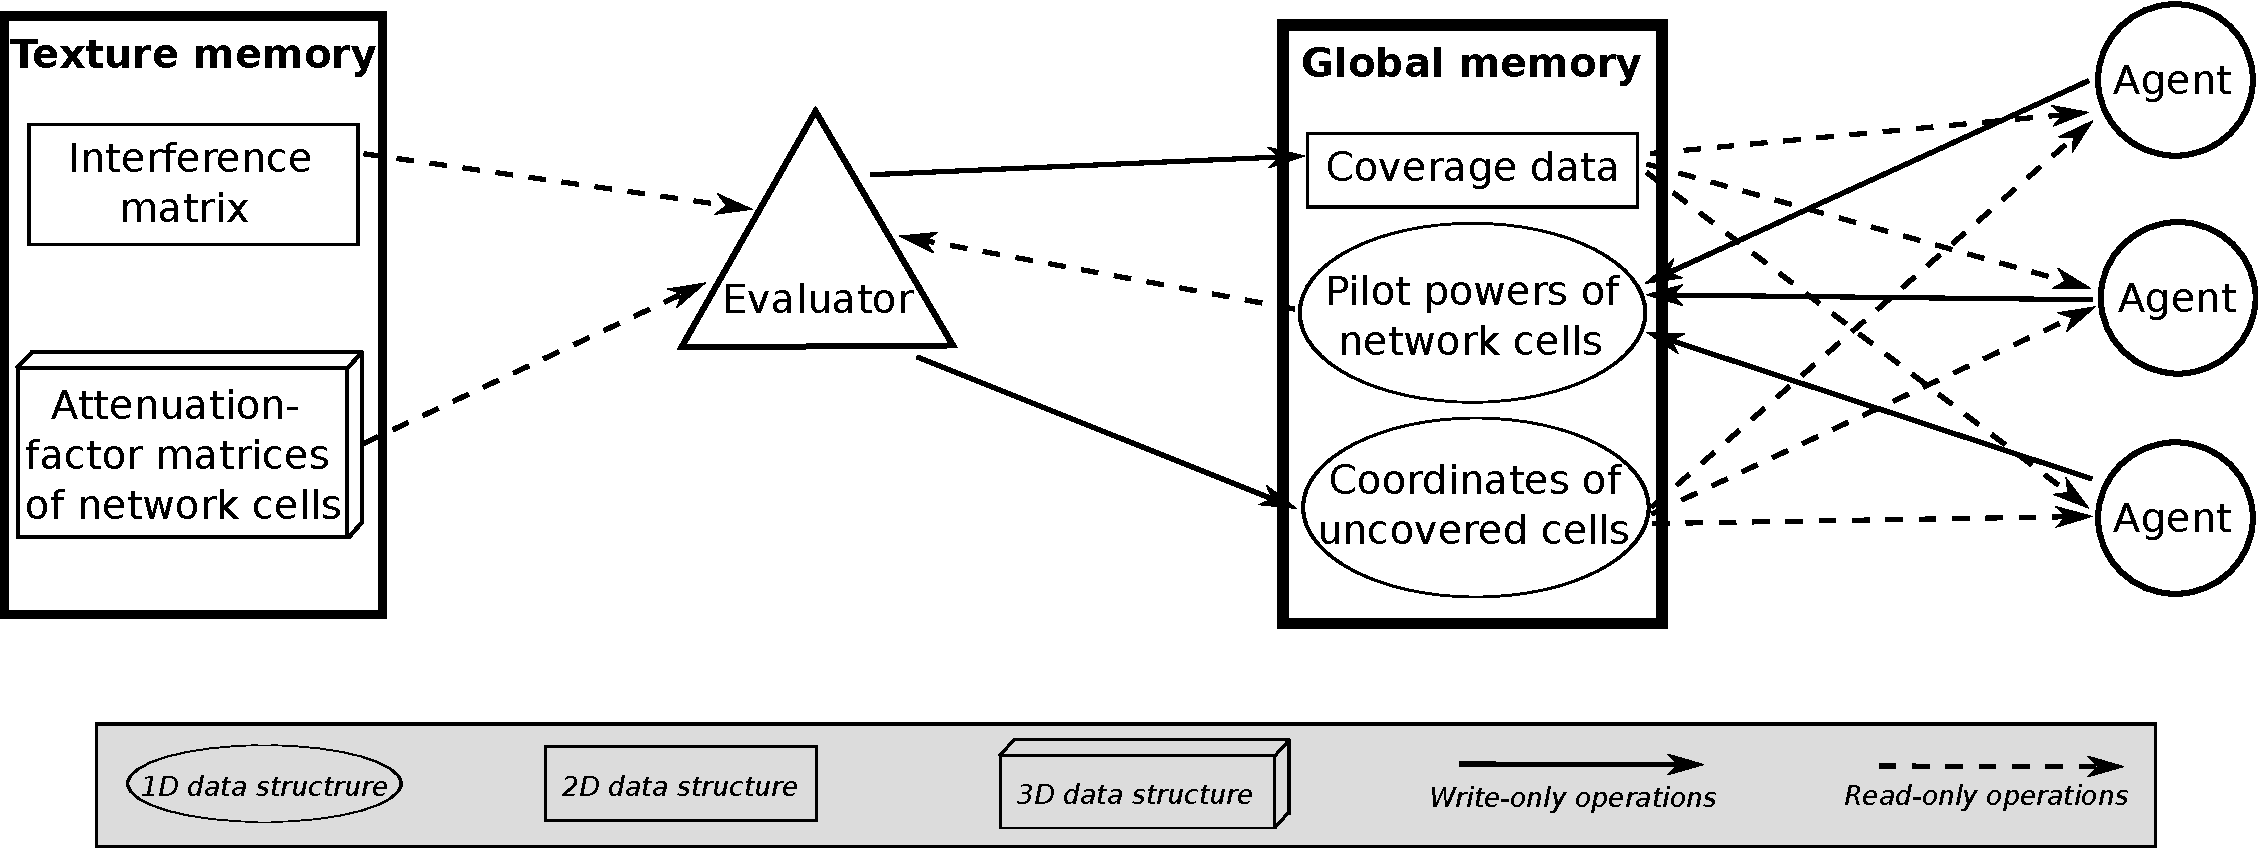
\includegraphics[width=1\textwidth]{06-experimental_evaluation-service_coverage/img/architecture}

\caption{Architecture of the parallel, agent-based optimization system on GPU.\emph{\label{fig:06-Architecture_of_the_system_on_GPU}}}
\end{figure}



\subsubsection{Objective-function evaluation}

The evaluator represents a central component of the optimization system.
It reacts to the pilot-power changes by recalculating the objective-function
value. Recall that the objective-function evaluation involves the
radio-coverage prediction of the service area and the calculation
of the total pilot power used by the cells in the target network.

After a short initialization, during which the attenuation-factor
matrices of all the cells and the interference matrix are calculated,
the evaluator computes the coverage of the service area based on the
pilot powers supplied as the initial solution. Initial solutions are
randomly generated from valid pilot-power settings that conform to
the full coverage constraint.

The evaluator also maintains a special part of the memory (see ``Coordinates
of uncovered cells'' in Figure~\ref{fig:06-Architecture_of_the_system_on_GPU})
that is intended for registering uncovered areas, i.e., $\overline{A_{\mathrm{covered}}}$.
If Equation (\ref{eq:06-Coverage_constraint}) does not hold, the
``special'' agents randomly select a location from this portion
of memory so that a valid solution may be reached again.

It is worth mentioning that the evaluator itself has no influence
in the optimization process from a quality point-of-view. Its task
is to provide feedback and updated information to the agents that
move through the service area. From a performance point-of-view, the
importance of the evaluator is significant, as it will be shown in
the following sections.

\bigskip{}


The evaluation of the objective function was completely implemented
on the GPU using OpenCL (see Section~\ref{sub:02-OpenCL}). The reason
behind this decision is the impact objective-function evaluation has
on the performance of the optimization system as a whole, as discussed
in Section~\ref{sub:02-Black_box_optimization}. The implementation
of the agents is also based on the GPU, which drastically reduces
the number of data transfers between CPU and GPU, since all problem
elements are available on the GPU during the optimization process.
Consequently, careful memory utilization and organization are critical
to successfully accommodate all involved problem elements on the GPU,
the memory of which is significantly smaller than the RAM available
in desktop computers.


\subsubsection{Autonomous agents}

The agents apply the pilot-power changes only considering local information.
Each of them encapsulates a set of steps that is consistently applied
as it randomly moves through the service area of the network. Whenever
an agent arrives at a new location, the set of covering cells is calculated,
i.e., $C_{m}$.

The step set an agent applies following this point is directly related
to $\vert C_{m}\vert$, whereas its movement is determined by $\vert\overline{A_{\mathrm{covered}}}\vert$,
i.e., the area without service coverage.

The behavior of an agent is dictated by the pseudo-code shown in Algorithm~\ref{alg:07-Agent-behavior}.
The first four steps are responsible for guiding its movements. The
coordinates are randomly selected from two sets, $A_{\mathrm{total}}$
and $\overline{A_{\mathrm{covered}}}$. Only ``special'' agents
may move to a location without service coverage, and they apply the
step set $SS_{0}$ for as long as the solution is not valid. The portion
of ``special'' agents used for correcting a solution is a parameter
of the optimization process. During the following steps of Algorithm~\ref{alg:07-Agent-behavior},
the agent applies step sets $SS_{0}$ and $SS_{1}$ based on the number
of cells in $C_{m}$.

\begin{algorithm}
\centering

\caption{Pseudo-code representing the behavior of an agent.\textit{\label{alg:07-Agent-behavior}}}


\begin{algorithmic}
\Repeat
	\If{$is\_special\_agent()$ $\mathbf{and}$ $\overline{A_{\mathrm{covered}}}>0$}
		\State $l \gets pick\_random\_location(\overline{A_{\mathrm{covered}}})$
	\Else
		\State $l \gets pick\_random\_location(A_{\mathrm{total}})$
	\EndIf
	\State $move(l)$
	\If{$\vert C_{m}\vert=0$}
		\State $apply(SS_{0})$
	\Else
		\If{$\vert C_{m}\vert\ge 1$}
			\State $apply(SS_{1})$
		\EndIf
	\EndIf
\Until{$stopping\_criterion()$}
\end{algorithmic}
\end{algorithm}


If the current location of the agent is not covered by any cell, i.e.,
$\vert C_{m}\vert=0$, the step set $SS_{0}$ is applied (see Algorithm~\ref{alg:07-Agent_step_set_0}).
At the beginning, the cell with the lowest path loss, $c'$, that
may cover a UE at this location, is selected. If several cells have
the same $l_{cm}^{\downarrow}$ value, one of them is randomly chosen.
Once $c'$ is uniquely identified, the agent changes its pilot power
by $inc\_rate$~dB.

\begin{algorithm}
\centering

\caption{Pseudo-code representing the step set $SS_{0}$, which is applied
by the agents in areas without service coverage.\textit{\label{alg:07-Agent_step_set_0}}}


\begin{algorithmic}
\Repeat
	\State $c'\gets cell\_with\_min\_path\_loss(m)$
	\State $p_{c'}\gets adjust\_power(c',inc\_rate)$
\Until{$p_{c'}\in P_{c'}$}
\end{algorithmic}
\end{algorithm}


\begin{algorithm}
\centering

\caption{Pseudo-code representing the step set $SS_{1}$, which is applied
by the agents in areas with service coverage.\label{alg:07-Agent_step_set_1}}


\begin{algorithmic}
\Repeat
	\State $c'\gets pick\_random\_cell(C_{m})$
	\State $p_{c'}\gets adjust\_power(c',dec\_rate)$
\Until{$p_{c'}\in P_{c'}$}
\end{algorithmic}
\end{algorithm}


The step set $SS_{1}$, the pseudo-code of which is listed in Algorithm~\ref{alg:07-Agent_step_set_1},
is applied if the location of the agent is under the coverage of one
or more cells, i.e., $\vert C_{m}\vert\ge1$. The first step randomly
selects a cell from the set $C_{m}$, followed by a decrease of the
pilot power of cell $c'$. This practice keeps the coverage constraint
valid over $A_{\mathrm{total}}$, although it might potentially break
it on other areas. Ideally, every pixel of the geographical area has
to be covered by exactly one network cell, although this is just a
representation of a perfect solution that is unreachable because of
irregularities in the network topology and the terrain.

In both step sets, $SS_{0}$ and $SS_{1}$, the agent makes sure that
the new pilot power setting, $p_{c'}$, is an element of $P_{c'}$.
If this is not the case, cell $c'$ is discarded and another cell
is repeatedly selected at the beginning of both step sets, until this
condition is satisfied.

The values $inc\_rate$ and $dec\_rate$ are configurable parameters
that should be set before starting the optimization process. They
indicate the relative adjustment (expressed in dB) of the pilot power
of cell $c'$. On the one hand, lowering the pilot power of a cell
decreases the interference it creates within its coverage area and
those of their neighbors. Since the $\mathrm{SINR}(c,m)$ value increases
with lower interference, the coverage of $m$ may be achieved by a
neighbor cell with the same or lower pilot power. On the other hand,
increasing the pilot power of the cell with the minimum path loss
improves the coverage by evenly distributing the power among different
network cells. This cell is, on average, the nearest one to the location
of a UE $m$.

\bigskip{}


With the objective-function evaluation running on the GPU, a new performance
bottleneck appeared. The limitation factor in this case was the CPU-to-GPU
data transfers that occurred in each iteration of the optimization
process (see Section~\ref{sec:02-CUDA}).

The GPU kernel of the agents is launched as one thread block that
contains one thread per deployed agent. The thread block is organized
in a one-dimensional grid. The initial location of each agent is randomly
generated using the current system time as a random seed. Since OpenCL
provides no function for random-number generation, a simplified version
of Marsaglia's generator~\cite{Marsaglia_Seeds.for.random.number.generator:2003}
was implemented.

The analysis each agent does about the received signals at the current
location is saved into the shared memory of the thread block. It contains
the network cell and its pilot-power setting. Since both numbers are
of type \emph{short}, each of which takes up two bytes, there is enough
space in a 16~KB shared-memory block to allocate 4,096 agents. The
last step involves saving the new pilot powers into global memory.
This step is performed by only one of the threads within the thread
block in order to avoid memory-access conflicts. Updated pilot powers
are saved in negative form to indicate that coverage re-calculation
is needed for these cells. In case there are several updated pilot
powers for one network cell, the median is calculated and applied
as the new pilot power.

Even though coalesced access is not achieved by the GPU kernel of
the agents, its sole implementation provided enhanced performance.
This performance gain appears because of the lower number of data
transfers between the CPU and the GPU, since most data are available
in global memory. Moreover, the GPU kernel also produces the truly
parallel behavior of the agents, as they all apply the pilot-power
changes at the same time.


\section{Simulations \label{sec:06-Simulations}}


\subsection{Test networks}

The test networks, Net$_{1}$, Net$_{2}$ and Net$_{3}$, are subsets
of the real radio network deployed by Telekom Slovenije, d.d. The
path-loss predictions were calculated using the radio-propagation
model presented in Section~\ref{sub:04-Radio_propagation_model}.
A DEM with a 25~m$^{2}$ resolution was used as the terrain-profile
data. The requirements for the coverage threshold, $\gamma^{\mathrm{cov}}$,
were provided by experts of the Radio Network department of Telekom
Slovenije, d.d.

Net$_{1}$ is deployed over a densely populated urban area. For this
reason, the value of $\gamma^{\mathrm{cov}}$ is lower here, since
network capacity is the dominating factor, whereas coverage is flexible
because of a larger cell density, i.e., more BSs per surface unit.
Net$_{2}$ represents a network deployed over a rural area, meaning
that the network capacity can be reduced at the cost of a better coverage,
since the user density is lower. The last network, Net$_{3}$, represents
a suburban area with a densely populated, but relatively small, downtown
center, where a compromise between the network capacity and the coverage
has to be achieved.

The second group of test networks, including Net$_{4}$, Net$_{5}$
and Net$_{6}$, is part of the publicly available MOMENTUM project~\cite{Momentum.project}.
Test network Net$_{4}$ represents the city of Berlin (Germany), Net$_{5}$
represents the city of The Hague (Netherlands), and Net$_{6}$ is
the largest network optimized in~\cite{Siomina:Minimum.pilot.power.for.service.coverage},
representing a reduced version of Net$_{4}$. All networks include
information about BS locations, path-loss predictions and realistic
antennas, which are part of the scenarios provided by the MOMENTUM
project.

Network configurations that represent what could be an initial-network
setup by common-planning standards~\cite{WCDMAforUMTS_RadioAccessForThirdGenerationMobileCommunications}
were produced using the attenuation-based approach. Such configurations
can be easily calculated by a network planner. Table~\ref{tab:06-Test_network_sizes}
lists the number of BSs and cells per test network, as well as the
size of the geographical area. Different network-parameter values
used during the simulations are shown in Table \ref{tab:06-Test_network_parameters}.

\begin{table}
\caption{Sizes of the test networks used for experimentation of the service-coverage
problem, in terms of equipment and geographical area.\emph{\label{tab:06-Test_network_sizes}}}


\centering

{\small{}}%
\begin{tabular}{ccccc}
\cmidrule{2-5} 
 & {\small{Number of base stations}} & {\small{Number of cells}} & {\small{Surface {[}km$^{2}${]}}} & {\small{Resolution {[}m$^{2}${]}}}\tabularnewline\addlinespace
\midrule
{\small{Net$_{1}$}} & {\small{26}} & {\small{77}} & {\small{100.00}} & {\small{25}}\tabularnewline
{\small{Net$_{2}$}} & {\small{8}} & {\small{23}} & {\small{306.25}} & {\small{25}}\tabularnewline
{\small{Net$_{3}$}} & {\small{45}} & {\small{129}} & {\small{405.00}} & {\small{25}}\tabularnewline
{\small{Net$_{4}$}} & {\small{65}} & {\small{193}} & {\small{56.25}} & {\small{50}}\tabularnewline
{\small{Net$_{5}$}} & {\small{12}} & {\small{36}} & {\small{16.00}} & {\small{50}}\tabularnewline
{\small{Net$_{6}$}} & {\small{50}} & {\small{148}} & {\small{56.25}} & {\small{50}}\tabularnewline
\bottomrule
\end{tabular}
\end{table}


\begin{table}
\caption{Network parameters of the test networks used for the service-coverage
problem.\emph{\label{tab:06-Test_network_parameters}}}


\centering

\begin{tabular}{cccc}
\cline{2-4} 
 & $p_{c}^{k}$ & $\mathrm{N}_{0}$ & $\gamma^{\mathrm{cov}}$\tabularnewline
\hline 
Net$_{1}$ & 15.00 W & 1.55$\cdot10^{-14}$ W & 0.010\tabularnewline
Net$_{2}$ & 19.95 W & 1.55$\cdot10^{-14}$ W & 0.020\tabularnewline
Net$_{3}$ & 15.00 W & 1.55$\cdot10^{-14}$ W & 0.015\tabularnewline
Net$_{4}$ & 19.95 W & 1.55$\cdot10^{-14}$ W & 0.010\tabularnewline
Net$_{5}$ & 19.95 W & 1.55$\cdot10^{-14}$ W & 0.010\tabularnewline
Net$_{6}$ & 19.95 W & 1.55$\cdot10^{-14}$ W & 0.010\tabularnewline
\hline 
\end{tabular}
\end{table}



\subsection{Parameter settings of the parallel-agent approach \label{sub:06-Algorithm_parameter_settings}}

The parameter settings for the optimization algorithm were determined
after some experimentation with the test networks. The parameter settings
for each test networks are listed in Table~\ref{tab:06-Parameter_settings}.

\begin{table}
\caption{Parameter settings of the parallel-agent approach for each test network.\emph{\label{tab:06-Parameter_settings}}}


\centering

\begin{tabular}{ccccc}
\cmidrule{2-5} 
 & Agents & $inc\_rate$ {[}dB{]} & $dec\_rate$ {[}dB{]} & Pilot-power changes\tabularnewline\addlinespace
\midrule
Net$_{1}$ & 16 & 0.2 & -0.1 & 10,000\tabularnewline
Net$_{2}$ & 16 & 0.2 & -0.1 & 10,000\tabularnewline
Net$_{3}$ & 16 & 0.2 & -0.1 & 10,000\tabularnewline
Net$_{4}$ & 6 & 1.0 & -0.1 & 10,000\tabularnewline
Net$_{5}$ & 2 & 1.0 & -0.1 & 10,000\tabularnewline
Net$_{6}$ & 6 & 1.0 & -0.1 & 10,000\tabularnewline
\bottomrule
\end{tabular}
\end{table}


Using a higher $inc\_rate$ than $dec\_rate$ reflects the behavior
of the agents when full coverage of the service area is not guaranteed.
In practice, areas without service coverage usually appear as irregular
islands. The stopping criteria were set by limiting the total number
of pilot-power changes an agent is allowed to make. The value was
set to 10,000, even though for some of the test networks the best
solutions were found in the first quarter of the experiment.

\bigskip{}


All experiments were performed on a multi-core Intel i7 2.67~GHz
desktop computer with 6~GB of RAM running a 64-bit Linux operating
system. The GPU hardware used was an ATI HD5570 with 1~GB of DDR3
RAM. The implementation language used was C, combined with OpenCL
and OpenMPI extensions.


\subsection{Results}

The results achieved by the parallel-agent approach, listed in Table~\ref{tab:06-Optimization_results},
improved the optimization objective significantly. They show that
the pilot-power usage was reduced in all networks while the service
area was kept under full coverage. Moreover, the parallel-agent solution
for Net$_{1}$ improved the attenuation-based setting by more than
300~\%. As for Net$_{2}$, the observed improvement is around 232~\%,
while the improvement for Net$_{3}$ is more than 170~\%. 

The last test network, Net$_{6}$, is the same as N6 in~\cite{Siomina:Minimum.pilot.power.for.service.coverage}.
When comparing these results to those of~\cite{Siomina:Minimum.pilot.power.for.service.coverage},
an improvement of almost 3~\% can be observed in the solution provided
by the parallel-agent approach, i.e., 0.778 against 0.759 for the
average pilot power of Net$_{6}$.

\begin{table}
\caption{Optimization results after applying two different approaches for solving
the service-coverage problem. All values are expressed in Watts.\emph{\label{tab:06-Optimization_results}}}


\centering

\begin{tabular}{crccrc}
\cmidrule{2-6} 
 & \multicolumn{2}{c}{Attenuation-based} &  & \multicolumn{2}{c}{Parallel agents}\tabularnewline\addlinespace
\cmidrule{2-3} \cmidrule{5-6} 
 & Total power & Average pilot power &  & Total power & Average pilot power\tabularnewline\addlinespace
\cmidrule{1-3} \cmidrule{5-6} 
Net$_{1}$ & 419.292 & 5.445 &  & 137.064 & 1.780\tabularnewline
Net$_{2}$ & 78.297 & 3.404 &  & 33.344 & 1.450\tabularnewline
Net$_{3}$ & 1,014.113 & 7.861 &  & 582.954 & 4.519\tabularnewline
Net$_{4}$ & 179.876 & 0.932 &  & 145.715 & 0.755\tabularnewline
Net$_{5}$ & 73.872 & 2.052 &  & 34.884 & 0.969\tabularnewline
Net$_{6}$ & 147.014 & 0.993 &  & 112.332 & 0.759\tabularnewline
\bottomrule
\end{tabular}
\end{table}



\subsection{Performance analysis}

The graphs shown in Figures~\ref{fig:06-Convergence_Net1}, \ref{fig:06-Convergence_Net2}
and~\ref{fig:06-Convergence_Net3} depict the convergence of the
parallel-agent approach after ten independent runs for test networks
Net$_{1}$, Net$_{2}$ and Net$_{3}$, respectively. Only feasible
solutions were plotted, i.e., the solutions that meet the full-coverage
constraint. Unfeasible solutions were marked with a value of inferior
quality than the worst solution found: 428 for Net$_{1}$, 129 for
Net$_{2}$, and 1,435 for Net$_{3}$.

From the graphs of Net$_{1}$ (see Figure~\ref{fig:06-Convergence_Net1})
and Net$_{2}$ (see Figure~\ref{fig:06-Convergence_Net2}), a good
initial convergence can be observed. This is followed by a steady
improvement of the intermediate solutions. In Net$_{1}$, no additional
solution improvement is noticed towards the end of the optimization
process. This fact suggests that the stopping criteria is suitable
for this problem instance. A similar situation is observed for Net$_{2}$
that also shows a flat profile towards the end. From the graph of
Net$_{3}$ (see Figure~\ref{fig:06-Convergence_Net3}), a slower
initial convergence, followed by a steady improvement of intermediate
solutions and no significant solution enhancement towards the end,
can be observed. This convergence profile suggests that this problem
instance presents a more difficult optimization case than for Net$_{1}$
and Net$_{2}$. Indeed, this is the largest test network in terms
of surface area. However, further investigation is needed to confirm
this hypothesis. Nevertheless, the parallel-agent approach improved
the pilot-power usage of this test network by almost 75~\%.

\begin{figure}[h]
\centering

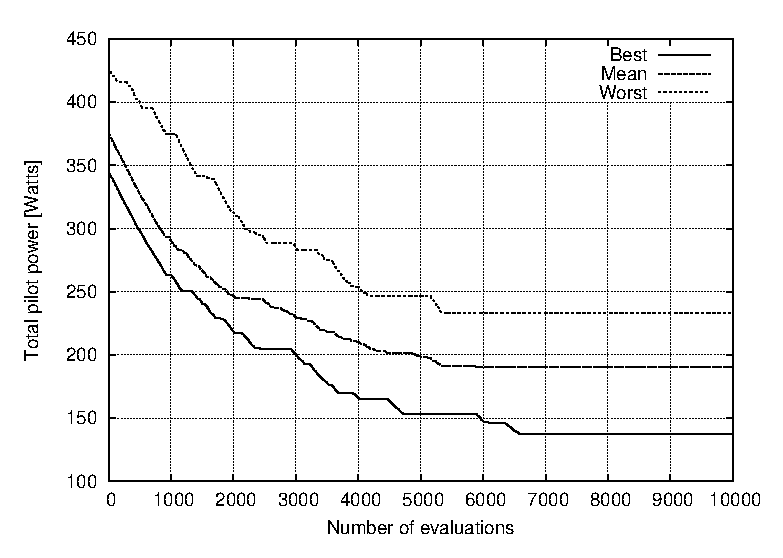
\includegraphics[width=0.7\textwidth]{06-experimental_evaluation-service_coverage/img/convergence_first}

\caption{Convergence profile of the parallel-agent approach for the test network
Net$_{1}$, deployed over an urban area.\emph{\label{fig:06-Convergence_Net1}}}
\end{figure}


\begin{figure}[h]
\centering

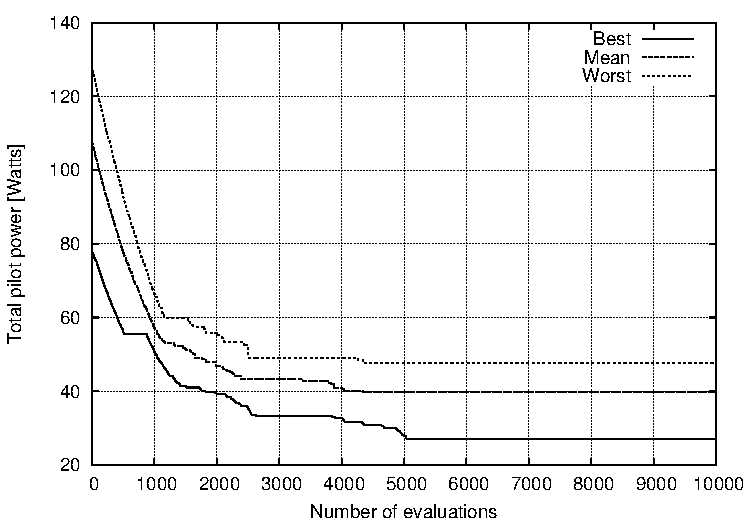
\includegraphics[width=0.7\textwidth]{06-experimental_evaluation-service_coverage/img/convergence_second}

\caption{Convergence profile of the parallel-agent approach for the test network
Net$_{2}$, deployed over a rural area.\emph{\label{fig:06-Convergence_Net2}}}
\end{figure}


\begin{figure}[h]
\centering

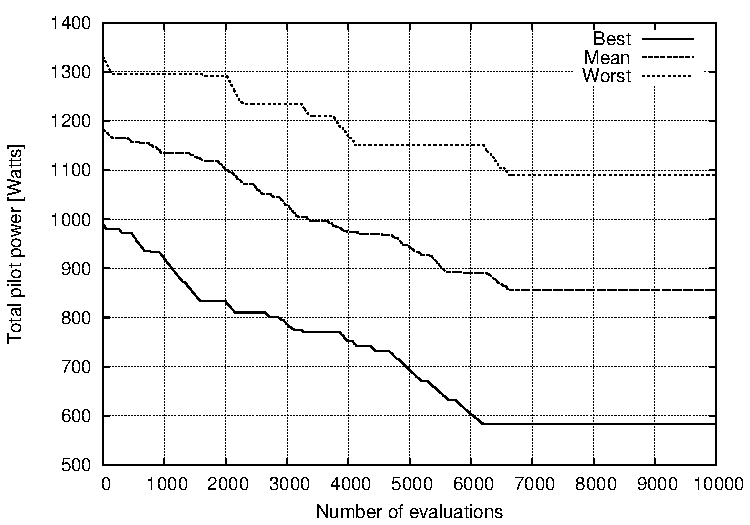
\includegraphics[width=0.7\textwidth]{06-experimental_evaluation-service_coverage/img/convergence_third}

\caption{Convergence profile of the parallel-agent approach for the test network
Net$_{3}$, deployed over a suburban area.\emph{\label{fig:06-Convergence_Net3}}}
\end{figure}


\bigskip{}


In the following, the speed-performance analysis of the experimental
simulations is presented. This analysis covers the running times during
the optimization of the first three test networks, i.e., Net$_{1}$,
Net$_{2}$ and Net$_{3}$. The running times were measured for each
implementation, and the average times, calculated after ten independent
runs, are given. The number of pilot-power changes per agent was limited
to 1,000, while all other algorithm parameters were kept at the same
values as in Section~\ref{sub:06-Algorithm_parameter_settings}.

Table~\ref{tab:06-Performance_analysis} lists the average wall-clock
times in seconds for the different implementations and test networks.
The implementations include: the CPU-MPI implementation that consists
of objective-function evaluation on CPU and parallel agents over MPI,
the GPU-MPI implementation that consists of objective-function evaluation
on GPU and parallel agents over MPI, and the GPU-GPU implementation
that consists of objective-function evaluation and parallel agents
on the same GPU. The CPU-MPI implementation is the basis for the speedup
calculation of the other two implementations.

The function evaluation on the GPU that communicates with the agents
over MPI provides the second measured setup. The evaluator implementation
takes advantage of shared memory for thread collaboration within a
thread block and texture memory for constant elements, as is it was
explained in Section~\ref{sub:04-GPU_worker_implementation}. Still,
the speedup is considerable but improvable, since numerous data transfers
between CPU and GPU are needed for the agents to access optimization-related
information. The last result set presents measurements for the complete
GPU implementation, including objective-function evaluation and agents
on the same device. The improved speedup delivered by this combination
highlights the impact that CPU-to-GPU memory transfers have on the
overall system performance. This fact is supported by the second and
third measured setups, the speedups of which exhibit, on average,
a four-fold improvement. It is also interesting to note how the speedup
gain increases with the problem-instance size. This fact confirms
that larger problem instances have a greater benefit from a parallel
implementation in terms of computational time.

\begin{table}
\caption{Wall-clock times (in seconds) and speedup factors for the different
implementations of the objective-function evaluation and the parallel
agents, as measured during the experimentation of the service-coverage
problem.\label{tab:06-Performance_analysis}}


\centering

\begin{tabular}{cccccccc}
\cmidrule{2-8} 
 & \multicolumn{1}{c}{CPU-MPI} &  & \multicolumn{2}{c}{GPU-MPI} &  & \multicolumn{2}{c}{GPU-GPU}\tabularnewline\addlinespace
\cmidrule{2-2} \cmidrule{4-5} \cmidrule{7-8} 
 & Avg. time {[}s{]} &  & Avg. time {[}s{]} & Speedup &  & Avg. time {[}s{]} & Speedup\tabularnewline\addlinespace
\cmidrule{1-2} \cmidrule{4-5} \cmidrule{7-8} 
Net$_{1}$ & 4,105 &  & 872 & 4.71 &  & 206 & 19.93\tabularnewline
Net$_{2}$ & 774 &  & 304 & 2.55 &  & 124 & 6.24\tabularnewline
Net$_{3}$ & 5,981 &  & 1,283 & 4.66 &  & 249 & 24.02\tabularnewline
\bottomrule
\end{tabular}
\end{table}



\section{Summary}

This chapter presented a novel optimization approach for solving the
well-known service-coverage problem in radio networks. The problem
addressed the full coverage of a geographical area using a minimum
amount of pilot power. The newly introduced parallel-agent approach
was successfully tested in six networks that represent real-world
scenarios. The experimental results show that the parallel-agent approach
is able to find better solutions than some heuristics, like the presented
attenuation-based approach. Moreover, the algorithm successfully tackled
larger networks, thus overcoming the obstacles of other state-of-the-art
optimization methods regarding problem-instance size~\cite{Siomina_Pilot.power.optimization:2004,Siomina:Minimum.pilot.power.for.service.coverage}.

Compared to a different optimization approach in the literature~\cite{Siomina:Minimum.pilot.power.for.service.coverage},
the solution-quality of the parallel-agent approach showed a quality
improvement. The proposed solutions, calculated for the same problem
instance as in~\cite{Siomina:Minimum.pilot.power.for.service.coverage},
were improved at the cost of a longer running time. It is worth mentioning
that it is feasible for the optimization algorithm to take a longer
time to reach the solution, since design problems, as the service-coverage
one, are usually solved offline. A comparison and analysis of the
performance of the radio-coverage prediction for real-world, radio-network
planning is later provided in Chapter~\ref{chap:08-Real-world_network_planning}.

Different implementations of the parallel-agent approach, combining
a serial version on CPU, parallel processes over MPI and GPU kernels,
were presented. In particular, GPU architectures enable the implementation
of parallel heuristics in a natural way while substantially improving
the computational-time performance. To the best of the author's knowledge,
the parallel-agent approach as presented in this chapter, has not
yet been described in the related literature.
